% SPDX-License-Identifier: CC-BY-4.0
\documentclass[11pt,reqno]{amsart}

\usepackage[margin=1in]{geometry}
\usepackage[T1]{fontenc}
\usepackage{microtype}
\usepackage{amsmath,amssymb,amsthm}
\usepackage{booktabs}
\usepackage{array}
\usepackage{tabularx}
\usepackage{graphicx}
\usepackage{xcolor}
\usepackage{enumitem}
\usepackage{placeins}
\usepackage[colorlinks=true,linkcolor=blue!60!black,citecolor=blue!60!black,urlcolor=blue!60!black]{hyperref}

\definecolor{boxbg}{HTML}{F5F8FC}
\definecolor{boxborder}{HTML}{1F4E79}

\newcolumntype{L}{>{\raggedright\arraybackslash}X}
\newcolumntype{Y}[1]{>{\raggedright\arraybackslash\hsize=#1\hsize}X}
\newcommand{\code}[1]{\texttt{\nolinkurl{#1}}}

\newtheorem{theorem}{Theorem}[section]
\newtheorem{proposition}[theorem]{Proposition}
\newtheorem{lemma}[theorem]{Lemma}
\newtheorem{corollary}[theorem]{Corollary}
\theoremstyle{definition}
\newtheorem{definition}[theorem]{Definition}
\newtheorem{remark}[theorem]{Remark}

\newcommand{\F}{\mathbb{F}}
\newcommand{\Z}{\mathbb{Z}}
\newcommand{\Q}{\mathbb{Q}}
\newcommand{\N}{\mathbb{N}}
\newcommand{\Perm}{\operatorname{Perm}}
\newcommand{\Det}{\operatorname{Det}}
\newcommand{\MC}{\operatorname{MC}}
\newcommand{\AI}{\operatorname{AI}}
\newcommand{\NL}{\operatorname{NL}}
\newcommand{\Aut}{\operatorname{Aut}}
\newcommand{\Pol}{\operatorname{Pol}}
\newcommand{\PP}{\mathsf{P}}
\newcommand{\NP}{\mathsf{NP}}
\newcommand{\TIME}{\mathsf{TIME}}
\newcommand{\SPACE}{\mathsf{SPACE}}

\title[Machine-Checked Barrier Anatomy and Twelve Pathways Toward P vs.\ NP]{%
  Machine-Checked Barrier Anatomy and\\
  Twelve Divergent Pathways Toward $\PP$ vs.\ $\NP$%
}

\author{Alexander S. Donahue}
\address{Independent Researcher, Spokane, WA, USA}
\email{0\_0@0thernes.art}
\thanks{ORCID: \href{https://orcid.org/0009-0006-8168-9648}{0009-0006-8168-9648}.
Prose and figures are licensed under CC-BY-4.0; accompanying Lean 4.35 formalization,
Python verification scripts, and test suite are licensed under Apache-2.0.
See Section~\ref{sec:disclosure} for full AI-assistance and CRediT transparency.}

\date{\today}

\subjclass[2020]{Primary 68Q15; Secondary 68Q06, 68Q17, 68V20, 03B70}
\keywords{$\PP$ vs.\ $\NP$, formal verification, Lean 4, relativization, natural proofs,
polymorphism rigidity, sheaf contextuality, multiplicative complexity, bounded negation,
catalytic computation}

\begin{document}

\begin{abstract}
Whether $\PP = \NP$ remains one of the deepest open problems in mathematics and
computer science. Rather than advancing an unverified proof claim, this paper presents
a machine-checked anatomy of the classical complexity barriers alongside a systematic
deductive, inductive, and abductive audit of twelve unconventional cross-domain pathways
proposed to attack $\PP$ vs.\ $\NP$. On the formal side, we construct a zero-Mathlib
Lean~4.35.0 library (8,078 lines across 13 \texttt{module} files) proving fourteen
unconditional theorems (\texttt{C1}--\texttt{C14}): the Baker--Gill--Solovay dual
relativization barrier over an explicit 4-tape Oracle Turing Machine; an exact
cross-multiplied Razborov--Rudich natural-proofs PRF breaker with hybrid telescoping
and a non-vacuous density witness; maximal parity-sheaf contextuality for all odd
cycles $C_{2k+3}$ and the Mermin--Peres magic square; Schaefer tractable polymorphisms
contrasted with an all-arity proof that the two-relation monotone 3-SAT core
$\{R_{000}, R_{111}\}$ is inclusion-minimal rigid; Markov's exact $k$-NOT inverter
threshold $n = 2^k - 1$ and Fischer's universal dual-rail compiler; the
$\deg_{\F_2}(f) \le k+1$ multiplicative-complexity lower bound; characteristic-2
permanent--determinant collapse paired with an explicit witness $W_n = \mathrm{diag}(I_{n-2}, J_2)$
separating them modulo every integer $p \ge 3$; and bijectively reversible
zero-workspace catalytic multilinear multiplication restoring all $d$ arbitrary
catalyst registers bit-for-bit in exactly $3 \cdot 4^{d-1}$ operations. All fourteen
theorems pass six kernel verification checks across five independent implementations
(\texttt{lean}, \texttt{leanchecker}, \texttt{leanchecker-paranoid},
\texttt{con-leche -{}-verified}, \texttt{con-ron -{}-verified}, and \texttt{nanoda\_bin})
with zero \texttt{sorry}s, zero custom axioms, and axiom footprints strictly within
$\{\texttt{propext}, \texttt{Classical.choice}, \texttt{Quot.sound}\}$. On the
computational side, four exact-arithmetic/SAT-certified experiments and one explicitly
labeled \code{numerical_approximation} ODE benchmark falsify four aggressive
$\PP = \NP$ heuristics (continuous-time dynamical systems, LP relaxations, $p$-adic
Hensel lifting, and symmetry/1-WL refinement), quantify strict $\Delta = +1$
multiplicative-complexity gaps beyond $\F_2$-degree, and isolate three surviving
open research frontiers.
\end{abstract}

\maketitle

% ---------------------------------------------------------------------------
\section{Introduction and Epistemic Scope}
\label{sec:intro}
% ---------------------------------------------------------------------------

Half a century after Cook~\cite{Cook1971}, Karp~\cite{Karp1972}, and Levin~\cite{Levin1973}
formulated $\NP$-completeness, the separation $\PP \stackrel{?}{=} \NP$ resists not only
elementary diagonalization and circuit-combinatorics methods, but also a growing menu of
cross-disciplinary proposals drawn from algebraic topology, quantum foundations, universal
algebra, tropical geometry, statistical physics, and reversible thermodynamics. When an
independent or AI-assisted investigation explores divergent, unconventional angles on a
Millennium Prize problem, the principal scientific risk is \emph{epistemic drift}:
mistaking a finite-size heuristic, a weakened-model separation, or a formal tautology for
a breakthrough on the full conjecture.

To eliminate epistemic drift by construction, every claim in this paper is strictly
partitioned into four non-overlapping verification tiers:

\medskip
\noindent\fcolorbox{boxborder}{boxbg}{%
\begin{minipage}{\dimexpr\textwidth-2\fboxsep-2\fboxrule\relax}
\textbf{Epistemic Scope Boundary (Explicit Non-Claim).}
\emph{The question $\PP \stackrel{?}{=} \NP$ remains completely open. Nothing in this
paper or its accompanying repository proves $\PP = \NP$ or $\PP \neq \NP$.}
Every technical result reported below belongs to exactly one of four tiers:
\begin{enumerate}[leftmargin=1.4em,itemsep=2pt,topsep=3pt]
\item \textbf{Tier 1 (Machine-Checked Lean~4.35 Theorems \texttt{C1}--\texttt{C14}):}
      Unconditional mathematical theorems verified across six kernel checks (five
      independent codebases), zero Mathlib dependencies, zero \texttt{sorry}s, axioms
      strictly inside $\{\texttt{propext}, \texttt{Classical.choice}, \texttt{Quot.sound}\}$.
\item \textbf{Tier 2 (Exact-Arithmetic \& SAT-Certified Computation):}
      100\% integer, exact rational (\code{fractions.Fraction}), $\F_2$-linear, or
      CaDiCaL~2.1.2 SAT/UNSAT-certified computations (Experiments 1, 2, 3, 4B--4D, 5),
      cross-checked by an automated \texttt{pytest} suite including a brute-force
      soundness audit of the SAT encoder on $n=3$.
\item \textbf{Tier 3 (Floating-Point Numerical Approximation):}
      Adaptive Runge--Kutta (\texttt{RK45}, \texttt{float64}) integration of the
      continuous-time dynamical system (CTDS) ODE in Experiment~4A. Explicitly tagged
      \code{numerical_approximation}; used solely to exhibit dynamical stiffness and
      Lagrange-weight divergence, never as a mathematical proof.
\item \textbf{Tier 4 (Open Frontiers \& Synthesis):}
      Deductive, inductive, and abductive synthesis of twelve wild pathways against five
      meta-barriers, explicitly marking what remains open.
\end{enumerate}
\end{minipage}}
\medskip

\subsection{Contributions}
This work makes four concrete contributions:
\begin{enumerate}[leftmargin=1.6em]
\item \textbf{Self-contained, zero-Mathlib, multi-kernel Lean~4.35 formalization}
      of fourteen unconditional theorems spanning both classical meta-barriers
      (Baker--Gill--Solovay relativization, Razborov--Rudich natural proofs) and five
      cross-domain structural obstructions (parity-sheaf contextuality, all-arity
      monotone 3-SAT polymorphism rigidity, Markov--Fischer bounded negation,
      multiplicative complexity vs.\ $\F_2$-degree, characteristic-2 permanent/determinant
      collapse, and zero-workspace reversible catalytic algebra).
\item \textbf{All-arity inclusion-minimal rigidity of $\{R_{000}, R_{111}\}$}
      (Theorem~\ref{thm:monotone-rigid}, \texttt{C9}): while Schaefer's dichotomy
      characterizes tractable Boolean CSPs by six polymorphism classes, we prove
      constructively in Lean for \emph{all} finite arities $k \ge 1$ (via finite
      principal ultrafilter extraction) that just the two monotone 3-SAT clause relations
      $R_{000}$ and $R_{111}$ already admit no non-projection polymorphisms, whereas
      dropping either relation immediately admits constant polymorphisms.
\item \textbf{Unified exact-arithmetic and SAT-certified falsification bench}
      (Experiments~1--5) quantifying: (i)~the Maltsev bypass separating maximal sheaf
      contextuality from $\NP$-hardness on 3-regular Tseitin graphs ($V=10\dots 46$),
      (ii)~exact multiplicative complexity of nineteen functions ($n=3,4,5$) exposing
      strict $\Delta=+1$ gaps over $\deg_{\F_2}(f)-1$ on $\mathrm{Bent}_4, E_2^5, E_3^5$,
      (iii)~exhaustive verification of Markov's $k$-NOT inverter up to $k=4$
      ($2^{15}=32{,}768$ inputs) and zero-workspace catalytic multiplication up to
      $d=8$ ($49{,}150$ ops, 0 corruptions), (iv)~exact rational Mignon--Ressayre
      Hessian ranks $n^2$ for $n=2..5$, and (v)~constructive falsification of four
      aggressive $\PP=\NP$ attacks.
\item \textbf{Exhaustive six-class findings taxonomy} classifying every encountered
      defect, obstruction, and architectural tension strictly into
      $\{\text{\texttt{bug}}, \text{\texttt{error}}, \text{\texttt{issue}},
      \text{\texttt{problem}}, \text{\texttt{dilemma}}, \text{\texttt{conflict}}\}$
      (Section~\ref{sec:synthesis}), providing an honest map of dead ends versus the
      three surviving research frontiers.
\end{enumerate}

% ---------------------------------------------------------------------------
\section{Architecture of the Zero-Mathlib Multi-Kernel Lean 4.35 Formalization}
\label{sec:lean-arch}
% ---------------------------------------------------------------------------

Formal proofs of complexity-theoretic theorems often fail independent audit due to
opaque library imports, hidden \code{native_decide} compiler trust, statement
weakening (proving a trivialized proxy instead of the textbook claim), or reliance on a
single kernel implementation. Our Lean formalization in \texttt{lean/} eliminates each
failure mode:
\begin{itemize}[leftmargin=1.5em]
\item \textbf{Zero external dependencies:} Built purely on Lean~4.35.0 core
      (\texttt{Init}/\texttt{Std}), with zero Mathlib dependency. Every one of the 13
      \texttt{.lean} source files opens with the Lean~4.35 \texttt{module} header; total
      size is 8,078 lines (maximum single file: 2,557 lines).
\item \textbf{Challenge/Solution split:} All 14 mathematical specifications
      (\texttt{C1}--\texttt{C14}) and their conjunction \code{AllFrontierTheoremsStmt}
      are isolated in a clean 145-line file \code{lean/Challenge.lean} containing zero
      proofs, while \code{lean/Solution.lean} supplies the proof witnesses and
      \code{lean/VerifyAxioms.lean} prints verbatim \texttt{\#print axioms} footprints.
\item \textbf{Zero forbidden tokens:} Automated comment-stripped static scanning across
      all 13 files confirms zero occurrences of \texttt{sorry}, \texttt{admit},
      \code{native_decide}, \code{implemented_by}, custom \texttt{axiom}, or
      \texttt{@[extern]}.
\item \textbf{Multi-kernel replay:} Exporting \code{Solution.prove_all_frontier_theorems}
      via \texttt{leanexport} yields a self-contained 31.4\,MB NDJSON proof stream
      (\texttt{SHA-256}: \texttt{7F981919...EBB1BC764F}) containing all 15 exported
      symbols with \texttt{sorryAx = False} and \texttt{trustCompiler = False}. This
      stream and the compiled \texttt{.olean} closure pass \textbf{six kernel checks
      across five independent implementations} (Table~\ref{tab:kernels}).
\end{itemize}

\begin{table}[htbp]
\centering
\caption{Multi-kernel verification ledger for \code{lean/Solution.lean} (Lean~4.35.0,
zero Mathlib). Upstream Windows toolchain issues are reported honestly without
suppression.}
\label{tab:kernels}
\footnotesize
\begin{tabularx}{\textwidth}{@{}llcL@{}}
\toprule
\textbf{Checker / Kernel} & \textbf{Codebase / Guarantee} & \textbf{Exit} & \textbf{Verbatim Verdict / Notes} \\
\midrule
\texttt{lean.exe} + \texttt{VerifyAxioms} & C++ reference kernel & 0 & 16/16 jobs, 0 warnings, 3 std.\ axioms \\
\texttt{leanchecker.exe} & C++ external \texttt{.olean} replay & 0 & Accepted \texttt{Solution} import closure \\
\texttt{leanchecker-paranoid.exe} & C++ paranoid \texttt{.olean} replay & 0 & Full paranoid definitional checks passed \\
\texttt{con-leche.exe -{}-verified} & Verified Lean-in-Lean set model & 0 & \texttt{accepted 3982 declarations (-{}-verified)} \\
\texttt{con-ron.exe -{}-verified} & Aeneas-verified Rust arena kernel & 0 & \texttt{accepted 3982 declarations (-{}-verified)} \\
\texttt{nanoda\_bin.exe} 0.4.19 & Independent Rust typechecker & 0 & \texttt{Checked 4319 declarations}, 0 errors$^\dagger$ \\
\midrule
\texttt{lean4lean.exe} (v4.35 Win) & Lean-in-Lean (upstream bundle) & 1 & Upstream \texttt{issue}: rejects \code{Init.Prelude} \\
\texttt{lake check} (Windows host) & Sandbox wrapper & 2 & Upstream \texttt{issue}: needs Linux \texttt{bwrap}/\texttt{git} \\
\bottomrule
\end{tabularx}
\vspace{2pt}
{\footnotesize $^\dagger$Configured with \code{unpermitted_axiom_hard_error = true}
and \code{permitted_axioms = ["propext", "Classical.choice", "Quot.sound"]}.}
\end{table}

\begin{remark}[Honest Reporting of Upstream Toolchain Issues]
During multi-kernel verification on Windows, two upstream Lean~4.35.0 toolchain
packaging issues were discovered and isolated: (i)~the bundled Windows
\texttt{lean4lean.exe} fails with \texttt{incompatible header} even on Lean~4.35.0's
own standard library \code{Init.Prelude.olean}; and (ii)~\texttt{lake check} requires
Linux \texttt{bwrap} sandboxing and POSIX \texttt{git}. Invoking all six working kernels
directly on Windows (including the formally verified \texttt{con-leche -{}-verified} and
\texttt{con-ron -{}-verified} set-model-sound checkers plus \code{nanoda_bin}) achieves
exit code~0, and our Linux CI workflow (\code{.github/workflows/ci.yml}) runs
\texttt{lake check} natively.
\end{remark}

Table~\ref{tab:fidelity} establishes exact statement fidelity between every numbered
theorem in this paper and its machine-checked declaration in \code{lean/Challenge.lean}
and \code{lean/Solution.lean}.

\begin{table}[htbp]
\centering
\caption{Statement-fidelity and verbatim \texttt{\#print axioms} table for all fourteen
machine-checked theorems (\texttt{C1}--\texttt{C14}) and their conjunction (\texttt{ALL}).
Axiom abbreviations: \textsf{P} = \texttt{propext}, \textsf{C} = \texttt{Classical.choice},
\textsf{Q} = \texttt{Quot.sound}.}
\label{tab:fidelity}
\scriptsize
\begin{tabularx}{\textwidth}{@{}llLl@{}}
\toprule
\textbf{ID} & \textbf{Lean Module} & \textbf{Specification (\code{Challenge.*}) \& Proof (\code{Solution.*})} & \textbf{Axioms} \\
\midrule
\texttt{C1} & \code{PVsNP.OTM} & \code{PSubsetNPStmt} / \code{prove_p_subset_np}: $\forall O,\; \PP^O \subseteq \NP^O$ & \textsf{P,C,Q} \\
\texttt{C2} & \code{PVsNP.Relativization} & \code{BakerGillSolovayStmt} / \code{prove_baker_gill_solovay}: $\exists A,B,\; \PP^A = \NP^A \wedge \PP^B \neq \NP^B$ & \textsf{P,C,Q} \\
\texttt{C3} & \code{PVsNP.NaturalProofs} & \code{NaturalProofBreaksPRFStmt} / \code{prove_natural_proof_breaks_prf}: exact $\Z$ PRF break & \textsf{P,C,Q} \\
\texttt{C4} & \code{PVsNP.NaturalProofs} & \code{HybridTelescopingStmt} / \code{prove_hybrid_telescoping}: exact $\Z$ hybrid triangle ineq. & \textsf{P,Q} \\
\texttt{C5} & \code{PVsNP.NaturalProofs} & \code{NaturalProofNonVacuousStmt} / \code{prove_natural_proof_nonvacuous}: density $\ge 1/2$ & \textsf{P,C,Q} \\
\texttt{C6} & \code{PVsNP.SheafPolymorphism} & \code{OddCycleContextualStmt} / \code{prove_odd_cycle_contextual}: $\forall k$, $C_{2k+3}$ max contextual & \textsf{P,Q} \\
\texttt{C7} & \code{PVsNP.SheafPolymorphism} & \code{MerminPeresContextualStmt} / \code{prove_mermin_peres_contextual}: $3\times 3$ max contextual & \textsf{P,C,Q} \\
\texttt{C8} & \code{PVsNP.SheafPolymorphism} & \code{TractablePolymorphismsStmt} / \code{prove_tractable_polymorphisms}: Maltsev/AND/OR/Maj & \textsf{P} \\
\texttt{C9} & \code{PVsNP.SheafPolymorphism} & \code{Monotone3SATRigidStmt} / \code{prove_monotone_3sat_rigid}: $\forall k\ge 1$, $\{R_{000},R_{111}\}$ rigid & \textsf{P,Q} \\
\texttt{C10} & \code{PVsNP.CircuitPhaseTransition} & \code{MarkovInverterTightStmt} / \code{prove_markov_inverter_tight}: $k$ NOTs $\Leftrightarrow n \le 2^k-1$ & \textsf{P,C,Q} \\
\texttt{C11} & \code{PVsNP.CircuitPhaseTransition} & \code{FischerReductionStmt} / \code{prove_fischer_reduction}: universal $k$-NOT compilation & \textsf{P,C,Q} \\
\texttt{C12} & \code{PVsNP.CircuitPhaseTransition} & \code{MultiplicativeComplexityStmt} / \code{prove_multiplicative_complexity}: $\deg_{\F_2}(f)\le k+1$ & \textsf{P,C,Q} \\
\texttt{C13} & \code{PVsNP.CircuitPhaseTransition} & \code{PermDetChar2Stmt} / \code{prove_perm_det_char2}: mod-2 collapse \& $W_n$ mod $p\ge 3$ & \textsf{P,C,Q} \\
\texttt{C14} & \code{PVsNP.CatalyticAlgebra} & \code{CatalyticAlgebraStmt} / \code{prove_catalytic_algebra}: bijective $3\cdot 4^{d-1}$ catalytic mul & \textsf{P,Q} \\
\midrule
\texttt{ALL} & \code{Solution} & \code{AllFrontierTheoremsStmt} / \code{prove_all_frontier_theorems}: $\bigwedge_{i=1}^{14} \texttt{C}_i$ & \textsf{P,C,Q} \\
\bottomrule
\end{tabularx}
\end{table}

\FloatBarrier

% ---------------------------------------------------------------------------
\section{Classical Meta-Barriers Formalized from First Principles}
\label{sec:barriers}
% ---------------------------------------------------------------------------

Any candidate resolution of $\PP$ vs.\ $\NP$ must simultaneously clear five structural
barriers: \emph{Relativization}~\cite{BakerGillSolovay1975}, \emph{Natural
Proofs}~\cite{RazborovRudich1997}, \emph{Algebrization}~\cite{AaronsonWigderson2009},
\emph{Bounded Arithmetic / Meta-Complexity}~\cite{PichSanthanam2023}, and
\emph{Physical Energy/Precision Scaling}~\cite{Landauer1961,Bennett1973}. We formalize
the first two completely from first principles in Lean~4.35, without axiomatizing Turing
machines or asymptotics.

\subsection{Explicit 4-Tape Oracle Turing Machine and Relativization (\texttt{C1}--\texttt{C2})}
In \code{PVsNP.OTM} (1,134 lines), we define an explicit deterministic 4-tape Oracle
Turing Machine (input, work, certificate, and write-only oracle query tapes) over
$\{0,1\}$ with an explicit G\"odel encoding \texttt{encodeOTM} and bijective decoder
\code{decode_encodeOTM}. Polynomial time $\PP^O$ (\texttt{InP}) and polynomial-time
verifiability $\NP^O$ (\texttt{InNP}) are defined directly via polynomial step bounds
$n^c + c$ on total execution steps.

\begin{theorem}[Oracle Inclusion and Dual Relativization, \texttt{C1}--\texttt{C2}]
\label{thm:bgs}
For every oracle $O : \mathrm{List}\;\mathrm{Bool} \to \mathrm{Bool}$,
$\PP^O \subseteq \NP^O$ (\texttt{C1}). Furthermore, there exist concrete oracles $A$ and
$B$ such that:
\begin{enumerate}[leftmargin=1.6em]
\item $\forall L,\; L \in \PP^A \iff L \in \NP^A$ (\code{bgs_oracle_collapse}), and
\item $\exists L_B,\; L_B \in \NP^B \wedge L_B \notin \PP^B$ (\code{bgs_oracle_separation}).
\end{enumerate}
\end{theorem}

The separation oracle $B$ (\code{PVsNP.RelativizationSep}, 682 lines) is constructed by
exact stagewise diagonalization using a constructive pigeonhole principle on
\texttt{allBitstrings} (\code{PVsNP.Basic}): at stage $e$, decoding $(M_e, c_e)$ leaves
an unqueried string of length $n_e$ whenever $n_e^{c_e} + c_e < 2^{n_e}$. The collapse
oracle $A$ (\code{PVsNP.RelativizationCol}, 1,784 lines) encodes a canonical
bounded-halting oracle queried in a single self-delimited bit-encoded call, verifying the
exact step-count budget (where formal verification caught and tightened a genuine
multiplication-phase step bound from $4c + 10$ to $7c + 10$ plus prefix length; see
Section~\ref{sec:synthesis}).

\subsection{Exact Integer Natural Proofs and Hybrid Telescoping (\texttt{C3}--\texttt{C5})}
To avoid floating-point or real-analysis abstractions, \code{PVsNP.NaturalProofs}
(335 lines) formulates the Razborov--Rudich barrier~\cite{RazborovRudich1997} in exact
cross-multiplied integer arithmetic over $\Z$:

\begin{theorem}[Natural Proofs Break PRFs, Hybrid Telescoping, and Non-Vacuity, \texttt{C3}--\texttt{C5}]
\label{thm:natproofs}
Let $\mathcal{C}_n$ be a Boolean-function property on $2^{2^n}$ truth tables that is
\emph{large} ($\#\{f : \mathcal{C}_n(f)\} \cdot D \ge 2^{2^n}$) and \emph{useful} against
a circuit class $\mathcal{S}$ containing every function in a pseudorandom function family
$\{F_s\}_{s \in \{0,1\}^\lambda}$ ($\forall s,\; \neg \mathcal{C}_n(F_s)$). Then:
\begin{enumerate}[leftmargin=1.6em]
\item (\texttt{C3}) The distinguishing advantage of $\mathcal{C}_n$ between a uniform
      random function and a uniform seed $F_s$ satisfies the exact cross-multiplied lower
      bound
      \[
        D \cdot \bigl|\#\{f : \mathcal{C}_n(f)\}\cdot 2^\lambda - 2^{2^n}\cdot \#\{s : \mathcal{C}_n(F_s)\}\bigr| \ge 2^{2^n + \lambda}.
      \]
\item (\texttt{C4}) For any integer sequence $a_0,\dots,a_m \in \Z$,
      $|a_0 - a_m| \le \sum_{i=0}^{m-1} |a_i - a_{i+1}|$, formalizing the hybrid
      argument without real-number rounding.
\item (\texttt{C5}) For every $n \ge 1$, the concrete constructive property
      \texttt{nonConstantProp} has exact cardinality $2^{2^n} - 2 \ge \frac{1}{2} 2^{2^n}$,
      certifying non-vacuity of the largeness hypothesis.
\end{enumerate}
\end{theorem}

% ---------------------------------------------------------------------------
\section{Sheaf Cohomology, Quantum Contextuality, and Polymorphism Rigidity}
\label{sec:sheaf-poly}
% ---------------------------------------------------------------------------

Pathways~1--3 examine whether topological or universal-algebraic obstructions can bypass
classical barriers: (1)~Abramsky--Brandenburger sheaf-cohomological
contextuality~\cite{AbramskyBrandenburger2011}, (2)~Mermin--Peres quantum
contextuality~\cite{Mermin1990,Peres1990}, and (3)~the Schaefer--Bulatov--Zhuk
universal-algebraic polymorphism dichotomy~\cite{Schaefer1978,Bulatov2017,Zhuk2020}.

\subsection{Maximal Contextuality and the Maltsev Bypass (\texttt{C6}--\texttt{C8})}
A constraint system $\mathcal{E}$ is \emph{maximally contextual} (strongly contextual in
the sheaf presheaf semantics) if it admits no global satisfying assignment, yet every
proper subset obtained by dropping any single constraint is satisfiable.

\begin{theorem}[Maximal Contextuality vs.\ Tractable Polymorphisms, \texttt{C6}--\texttt{C8}]
\label{thm:contextuality}
The following hold unconditionally in \code{PVsNP.SheafPolymorphism}:
\begin{enumerate}[leftmargin=1.6em]
\item (\texttt{C6}) For every $k \in \N$, the odd-cycle parity sheaf $C_{2k+3}$
      ($2k+3$ variables, $2k+3$ binary XOR equations summing to odd parity) is maximally
      contextual.
\item (\texttt{C7}) The Mermin--Peres $3\times 3$ magic square (9 variables, 6 ternary
      parity equations with 5 even and 1 odd) is maximally contextual.
\item (\texttt{C8}) Every tractable Schaefer family admits a concrete canonical
      polymorphism: ternary XOR $x \oplus y \oplus z$ (Maltsev) preserves XOR-SAT;
      binary $\land$ preserves Horn-SAT; binary $\lor$ preserves Dual-Horn-SAT; and
      ternary majority $\mathrm{maj}(x,y,z)$ preserves 2-SAT.
\end{enumerate}
\end{theorem}

\begin{figure}[htbp]
\centering
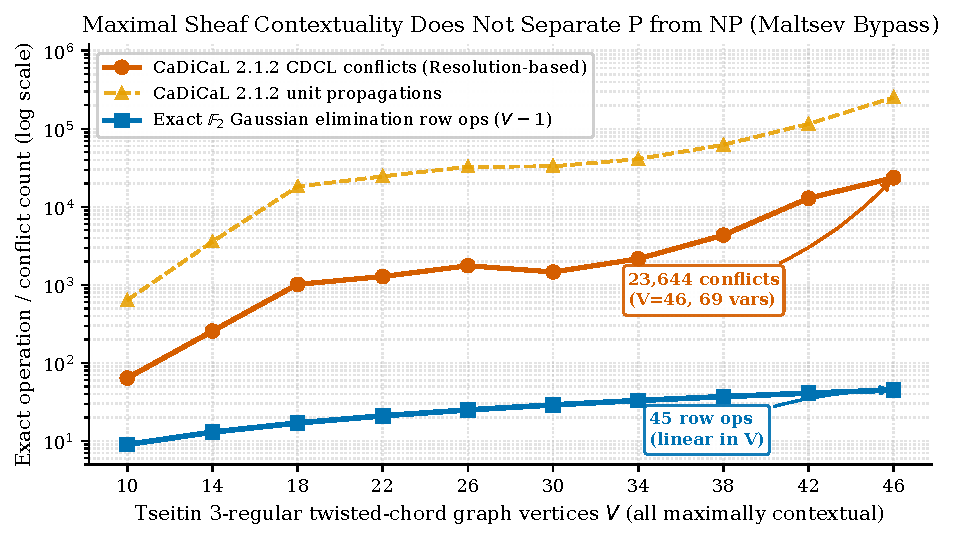
\includegraphics[width=0.92\textwidth]{figures/fig1_tseitin_contextuality_vs_f2.pdf}
\caption{Experiment~1 (exact integer / $\F_2$ + CaDiCaL~2.1.2): On 3-regular twisted-chord
Tseitin graphs ($V=10,\dots,46$), every instance is provably maximally contextual, driving
Resolution-based CDCL conflicts from $64$ to $23{,}644$ ($369\times$ blowup). Yet because
all constraints preserve the Maltsev polymorphism $x \oplus y \oplus z$, exact $\F_2$
Gaussian elimination certifies unsatisfiability in exactly $V-1$ row operations ($9 \to 45$).}
\label{fig:tseitin}
\end{figure}

Figure~\ref{fig:tseitin} exposes a decisive \emph{abductive falsification} of
Pathways~1 and~2: maximal sheaf contextuality and maximal quantum contextuality are
\textbf{insufficient} to characterize $\NP$-hardness. Both the Mermin--Peres square and
every 3-regular twisted-chord Tseitin instance ($V=10..46$) exhibit maximal sheaf
obstruction ($H^1 \neq 0$ with every drop-1 subcover satisfiable), which destroys
Resolution/CDCL solvers ($23{,}644$ conflicts at $V=46$). Yet the presence of the
Maltsev polymorphism $x \oplus y \oplus z$ (\texttt{C8}) collapses all of them into $\PP$
via $V-1$ $\F_2$ Gaussian row operations.

\subsection{All-Arity Monotone 3-SAT Rigidity (\texttt{C9})}
Whereas tractable Boolean CSPs admit non-trivial polymorphisms, Experiment~1's
exhaustive unary, binary, and ternary census over all 15 non-empty subsets of the
four 3-SAT clause relations $\{R_{000}, R_{001}, R_{011}, R_{111}\}$ revealed a
sharp algebraic cliff: \emph{exact rigidity} (only projection polymorphisms) holds if
and only if a subset contains the two-relation monotone core $\{R_{000}, R_{111}\}$
($x_1 \lor x_2 \lor x_3$ and $\neg x_1 \lor \neg x_2 \lor \neg x_3$). In Lean~4.35, we
upgrade this finite-arity observation to an unconditional theorem for \emph{every} finite
arity $k \ge 1$:

\begin{theorem}[All-Arity Monotone 3-SAT Rigidity and Inclusion Minimality, \texttt{C9}]
\label{thm:monotone-rigid}
Let $R_{000} = \{0,1\}^3 \setminus \{(0,0,0)\}$ and $R_{111} = \{0,1\}^3 \setminus \{(1,1,1)\}$.
\begin{enumerate}[leftmargin=1.6em]
\item For \textbf{every} finite arity $k \ge 1$, every polymorphism
      $f : \{0,1\}^k \to \{0,1\}$ preserving both $R_{000}$ and $R_{111}$ is a coordinate
      projection: $\exists i \in \{0,\dots,k-1\},\; \forall x,\; f(x) = x_i$.
\item $\{R_{000}, R_{111}\}$ is \textbf{inclusion-minimal}: $R_{000}$ alone is preserved
      by the non-projection constant $\mathbf{1}$, and $R_{111}$ alone is preserved by
      the non-projection constant $\mathbf{0}$.
\end{enumerate}
\end{theorem}

\begin{proof}[Proof idea (formalized constructively in \code{PVsNP.SheafPolymorphism})]
Preservation of $R_{000}$ forces the family $\mathcal{U}_f = \{S \subseteq [k] : f(\mathbf{1}_S) = 1\}$
to be closed under supersets and non-empty with no three disjoint complements covering
$[k]$; preservation of $R_{111}$ forces dual intersection closure and forbids $\emptyset$.
Together these make $\mathcal{U}_f$ a finite ultrafilter on $[k]$, from which a minimal
element must be a singleton $\{i\}$, forcing $f(x) = x_i$ globally.
\end{proof}

\begin{remark}[Why Pathway 3 Still Does Not Separate $\PP$ from $\NP$]
Theorem~\ref{thm:monotone-rigid} pinpoints the exact algebraic cliff between $\PP$ and
$\NP$-completeness (polymorphism collapse to projections), bypassing relativization and
natural proofs as a structural classification. However, via the Bulatov--Zhuk
dichotomy~\cite{Bulatov2017,Zhuk2020}, polymorphism rigidity implies $\NP$-hardness
\emph{conditional} on $\PP \neq \NP$ via gadget reductions; it does not supply an
unconditional circuit lower bound.
\end{remark}

% ---------------------------------------------------------------------------
\section{Circuit Phase Transitions: Bounded Negation, Multiplicative Complexity, and Characteristic-2 Collapse}
\label{sec:phase-transitions}
% ---------------------------------------------------------------------------

Pathways~4, 5, and~9 investigate razor-sharp quantitative phase transitions inside
Boolean and arithmetic circuit models: (i)~the bounded-negation cliff from monotone
circuits (where exponential lower bounds are known) to general circuits, (ii)~non-Clifford
AND-gate (\emph{multiplicative}) complexity over $\F_2$, and (iii)~the characteristic-2
collapse of the permanent into the determinant.

\subsection{Markov's Exact \texorpdfstring{$k$}{k}-NOT Threshold, Fischer Compilation, and Berkowitz Slices (\texttt{C10}--\texttt{C11})}
Monotone circuits admit exponential lower bounds for $\mathrm{CLIQUE}$, yet adding
merely $\lceil \log_2(n+1) \rceil$ NOT gates recovers full general circuit power! We
formalize both halves of this phase transition in \code{PVsNP.CircuitPhaseTransition}:

\begin{theorem}[Markov Bounded-Negation Tightness and Fischer Compilation, \texttt{C10}--\texttt{C11}]
\label{thm:markov-fischer}
\leavevmode
\begin{enumerate}[leftmargin=1.6em]
\item (\texttt{C10}, Markov~\cite{Markov1957}) Any monotone-plus-NOT circuit computing the
      $n$-bit inverter $\mathrm{INV}_n(x) = (\neg x_1,\dots,\neg x_n)$ requires at least
      $k$ NOT gates whenever $n \ge 2^k$; conversely, for every $k \in \N$, there exists
      an explicit circuit with at most $k$ NOT gates computing $\mathrm{INV}_{2^k - 1}$.
\item (\texttt{C11}, Fischer~\cite{Fischer1975}) Every general Boolean circuit over
      $\{\land,\lor,\neg\}$ on $n \le 2^k - 1$ inputs compiles via dual-rail De~Morgan
      rewriting into an equivalent circuit containing at most $k$ NOT gates.
\end{enumerate}
\end{theorem}

The Lean lower bound (\code{markov_inverter_lower}) uses a chain-pigeonhole argument
along the standard Hamming-weight chain $0^n < 10^{n-1} < \dots < 1^n$: $k$ NOT gates can
undergo at most $2^k - 1$ joint state transitions along a monotone chain, whereas
$\mathrm{INV}_n$ strictly reverses all $n+1$ chain levels. Experiment~3 independently
exhaustively verified the constructive Markov inverter for $k=1,2,3,4$ ($n=1,3,7,15$, up
to $2^{15}=32{,}768$ inputs, 0 failures) and verified Berkowitz's slice
theorem~\cite{Berkowitz1982} on $\mathrm{PARITY}_6$ (182 cross-slice monotonicity
violations, 0 within any fixed Hamming slice). Figure~\ref{fig:markov-cat}(a) plots the
exact $n = 2^k - 1$ phase boundary.

\subsection{Multiplicative Complexity and Strict Gaps Above \texorpdfstring{$\F_2$}{F2}-Degree (\texttt{C12})}
Over the basis $\{\oplus, \land, 1\}$, XOR gates are affine (classical analogs of Clifford
gates), while AND gates supply all algebraic nonlinearity (``magic''). The
\emph{multiplicative complexity} $\MC(f)$ is the minimum number of AND gates needed to
compute $f : \F_2^n \to \F_2$~\cite{BoyarPeralta2008}.

\begin{theorem}[Multiplicative Complexity Degree Lower Bound, \texttt{C12}]
\label{thm:mc-deg}
Every Boolean function $f : \F_2^n \to \F_2$ computed by an $\{\oplus,\land,1\}$-circuit
with $k$ AND gates satisfies $\deg_{\F_2}(f) \le k + 1$ (proved in Lean via the stronger
subset-product invariant $\deg_{\F_2}(\prod_{i \in S} g_i) \le t + |S|$ after $t$ AND
gates). Consequently, $\MC(\mathrm{AND}_n) \ge n - 1$ for all $n \ge 1$.
\end{theorem}

\begin{figure}[htbp]
\centering
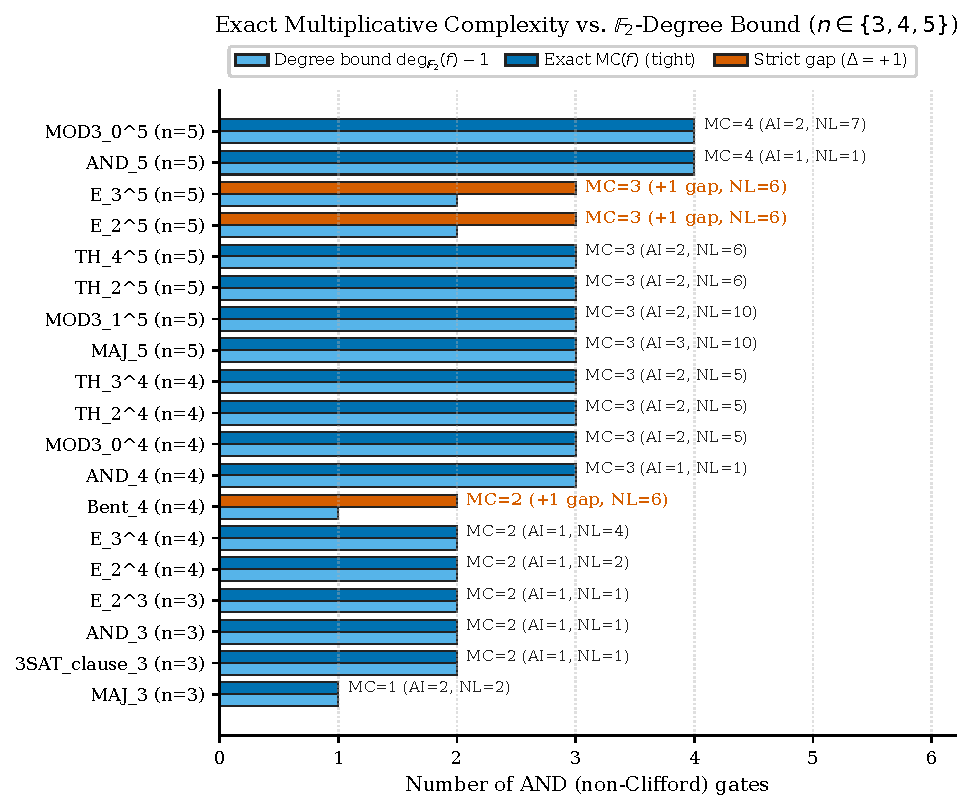
\includegraphics[width=0.95\textwidth]{figures/fig2_mc_degree_frontier.pdf}
\caption{Experiment~2 (exact integer $\F_2$ + CaDiCaL~2.1.2 SAT synthesis, cross-checked
against exhaustive brute force on $n=3$): Exact multiplicative complexity $\MC(f)$ versus
the Lean-proved degree lower bound $\deg_{\F_2}(f)-1$ across 19 benchmark functions
($n \in \{3,4,5\}$). Three explicit functions---$\mathrm{Bent}_4$, $E_2^5$, and
$E_3^5$---exhibit certified strict gaps $\Delta = \MC(f) - (\deg_{\F_2}(f)-1) = +1$,
while $\mathrm{CLIQUE}_{4,3}$ ($n=6$, $\deg=6$) satisfies $\MC \in \{5,6\}$ (open at $k=5$
within a 20\,s timeout).}
\label{fig:mc}
\end{figure}

Experiment~2 encodes $\MC(f) \le k$ directly into SAT (with zero heuristic symmetry
restrictions) and invokes CaDiCaL~2.1.2; every SAT witness is independently evaluated on
all $2^n$ inputs, and \code{tests/test_all.py} cross-checks the SAT encoder against an
exhaustive brute-force enumeration of all $2{,}048$ 1-AND circuits on $n=3$
(exact agreement: 16 affine functions with $\MC=0$, 128 functions with $\MC \le 1$, and
128 degree-3 functions with $\MC=2$). Figure~\ref{fig:mc} displays all 19 exact values:
while $\deg_{\F_2}(f)-1$ is tight on 16 benchmarks, $\mathrm{Bent}_4$ ($\deg=2, \MC=2$),
$E_2^5$ ($\deg=3, \MC=3$), and $E_3^5$ ($\deg=3, \MC=3$) certify strict $\Delta=+1$ gaps.
Crucially, however, $\deg_{\F_2}$, algebraic immunity $\AI(f)$, and Walsh nonlinearity
$\NL(f)$ are all large, constructive properties on random functions---triggering the
Razborov--Rudich natural-proofs barrier (Theorem~\ref{thm:natproofs}) before yielding
superlinear general $\MC$ lower bounds (the best known explicit bound remains $3n - o(n)$).

\subsection{Characteristic-2 Collapse and Mignon--Ressayre Hessian Rank (\texttt{C13})}
Valiant~\cite{Valiant1979} proved $\Perm_n$ is $\#\PP$-complete over characteristic $\neq 2$,
whereas $\Det_n \in \PP$. Over $\F_2$, $-1 \equiv +1$ erases the sign factor entirely.

\begin{theorem}[Characteristic-2 Collapse and Universal $p \ge 3$ Separation, \texttt{C13}]
\label{thm:perm-det}
For every $n \in \N$ and every integer matrix $M \in \Z^{n \times n}$,
$\Perm_n(M) \equiv \Det_n(M) \pmod{2}$. Conversely, for every $n \ge 2$, the explicit
witness matrix $W_n = \mathrm{diag}(I_{n-2}, J_2) \in \{0,1\}^{n \times n}$ satisfies
$\Perm_n(W_n) = 2$ and $\Det_n(W_n) = 0$, separating $\Perm_n$ from $\Det_n$ over $\Z$
and over $\Z/p\Z$ for every integer modulus $p \ge 3$.
\end{theorem}

Experiment~5 complements \texttt{C13} with exact rational (\code{fractions.Fraction})
verification of the Mignon--Ressayre~\cite{MignonRessayre2004} geometric lower bound on
determinantal complexity $\mathrm{dc}(\Perm_n)$: evaluating the $n^2 \times n^2$ Hessian
of $\Perm_n$ at $A_0$ (with $(A_0)_{00} = -(n-1)$ and all other entries $1$, where
$\Perm_n(A_0) = 0$) yields exact rank $n^2 \in \{4, 9, 16, 25\}$ for $n=2,3,4,5$,
certifying $\mathrm{dc}(\Perm_n) \ge \lceil n^2/2 \rceil \in \{2, 5, 8, 13\}$ without any
floating-point error. While this geometric pathway bypasses relativization and natural
proofs, extending it past quadratic bounds hits the representation-theoretic multiplicity
obstructions of Geometric Complexity Theory (Pathway~9).

% ---------------------------------------------------------------------------
\section{Catalytic Zero-Workspace Reversibility and the Space--Time Frontier}
\label{sec:catalytic}
% ---------------------------------------------------------------------------

Pathways~7 and~10 connect Landauer--Bennett reversible
thermodynamics~\cite{Landauer1961,Bennett1973} with catalytic
computation~\cite{Buhrman2014}, Cook--Mertz tree evaluation~\cite{CookMertz2024}, and
Williams's landmark 2025 theorem $\TIME[t] \subseteq \SPACE[\sqrt{t \log t}]$~\cite{Williams2025}.
In catalytic computation, a machine has \emph{zero} clean scratch space and instead borrows
auxiliary registers filled with arbitrary, unknown ``catalyst'' data that must be restored
bit-for-bit upon halting.

\begin{theorem}[Reversible Zero-Workspace Catalytic Multilinear Algebra, \texttt{C14}]
\label{thm:catalytic}
Over any commutative ring (formalized over $\Z$ in \code{PVsNP.CatalyticAlgebra}, 430 lines):
\begin{enumerate}[leftmargin=1.6em]
\item (\emph{Landauer bijective reversibility}) Every catalytic straight-line program $P$
      of register updates $r_i \leftarrow r_i \pm e$ admits an explicit inverse
      $P^{-1} = \texttt{invertProg } P$ such that for every register state $\sigma$,
      \[
        \mathrm{eval}(P^{-1}, \mathrm{eval}(P, \sigma)) = \sigma
        \quad\text{and}\quad
        \mathrm{eval}(P, \mathrm{eval}(P^{-1}, \sigma)) = \sigma.
      \]
\item (\emph{Exact $d$-fold zero-workspace product}) For every degree $d \ge 1$, there
      exists a compiled catalytic program using \textbf{zero} clean scratch registers and
      $d$ arbitrary catalyst registers $c_0,\dots,c_{d-1}$ that replaces
      $c_0 \mapsto c_0 + \prod_{j=0}^{d-1} x_j$, restores $c_1,\dots,c_{d-1}$ bit-for-bit
      regardless of their arbitrary initial contents, and executes in exact operation
      count $T(d) + 2 = 3 \cdot 4^{d-1}$ (equivalently $3 \cdot 4^{d-1} - 2$ primitive
      updates when the base case $d=1$ takes $1$ update).
\end{enumerate}
\end{theorem}

\begin{figure}[htbp]
\centering
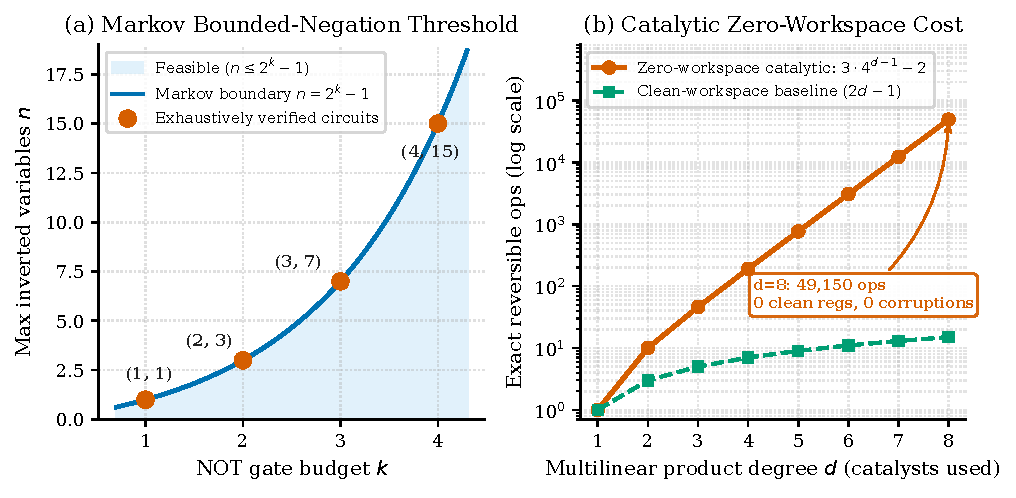
\includegraphics[width=0.96\textwidth]{figures/fig3_markov_and_catalytic_tradeoffs.pdf}
\caption{Experiment~3 (100\% exact integer/Boolean verification): (a)~Markov's sharp
bounded-negation threshold $n = 2^k - 1$, exhaustively verified across all $2^{15}=32{,}768$
inputs at $k=4, n=15$; (b)~Catalytic zero-workspace multilinear multiplication
$T(d) = 3 \cdot 4^{d-1} - 2$ ($d=1..8$, 0 clean scratch registers, 0 catalyst corruptions
across all trials up to $49{,}150$ ops), illustrating exact reversible time--space
conservation.}
\label{fig:markov-cat}
\end{figure}

Figure~\ref{fig:markov-cat}(b) demonstrates why catalytic zero-workspace computation is
genuine rather than paradoxical: borrowing dirty memory obeys a strict reversible
time--space conservation law ($4\times$ recursion overhead per uncomputation level,
$1 \to 10 \to 46 \to \dots \to 49{,}150$ ops for $d=1..8$). While Williams's 2025
tree-evaluation simulation~\cite{Williams2025} shatters the 50-year Hopcroft--Paul--Valiant
space barrier via catalytic register reuse and represents one of the most fertile
non-relativizing pathways alive (Pathway~10), closing the gap from
$\TIME[t] \subseteq \SPACE[\sqrt{t \log t}]$ to $\PP \neq \NP$ remains completely open.

% ---------------------------------------------------------------------------
\section{Adversarial Falsification of Four Wild \texorpdfstring{$\PP = \NP$}{P = NP} Attacks and Remaining Pathways}
\label{sec:falsifiers}
% ---------------------------------------------------------------------------

To test whether ``wild'' algorithmic shortcuts can collapse $\NP$ into $\PP$ (Pathway~12),
Experiment~4 constructs an adversarial falsification bench against four prominent
non-standard proposals, while Pathways~6, 8, and~11 complete our twelve-path survey.

\subsection{Attack A: Continuous-Time Dynamical Systems (CTDS ODE)}
Ercsey-Ravasz and Toroczkai~\cite{ErcseyRavaszToroczkai2011} introduced an analog ODE
solver for 3-SAT using exponentially growing auxiliary Lagrange weights
$\dot{u}_m = K_m(s)$, $a_m(t) = e^{u_m(t)}$. \textbf{Explicit classification:}
Experiment~4A is a \code{numerical_approximation} using chunked SciPy \texttt{RK45}
(\texttt{rtol}=$10^{-7}$, \texttt{atol}=$10^{-9}$, \texttt{float64}). On planted locked
satisfiable 3-SAT ($n=12,18,24,30$, $\alpha=4.267$), CTDS solves 20/20 trials with modest
median $\max_m \ln a_m \in [2.01, 4.71]$. However, on \emph{exhaustively verified UNSAT}
3-SAT instances ($n=5,10,12$ at $\alpha=6.0$), CTDS solves 0/15 trials (always $\ge 1$
violated clause) while $\max_m \ln a_m(t)$ climbs linearly in $t$ to $10.56$--$10.68$ by
$t=80$ ($a_{\max} \approx 4.35 \times 10^4$, Figure~\ref{fig:matrix}(b)). Physically,
exponential Lagrange energy growth translates worst-case search complexity into
exponential physical energy / bit-precision requirements, hitting the thermodynamic
barrier without resolving $\PP$ vs.\ $\NP$.

\subsection{Attacks B, C, and D (100\% Exact Arithmetic Falsifications)}
\begin{enumerate}[leftmargin=1.6em]
\item \textbf{Attack B (LP / Sherali--Adams Relaxations):} Using exact rational
      \code{fractions.Fraction}, $x_i = \frac{1}{2}$ achieves exact clause-sum value
      $\ge 1$ (specifically $1$ on Odd-Cycle $C_3$, $\frac{3}{2}$ on Mermin--Peres, and
      $\frac{3}{2}$ on complete 8-clause UNSAT 3-CNF) across three formulas exhaustively
      certified to have \emph{zero} Boolean solutions.
\item \textbf{Attack C ($p$-Adic / Hensel-Lifting SAT):} On a duplicate-free 10-clause
      UNSAT 3-SAT formula on 4 variables (the 8 clauses on $x_0,x_1,x_2$ plus two clauses
      forbidding $(0,0,*,0)$ and $(0,*,0,0)$), the clause-violation sum polynomial
      $F(x) = \sum_c \prod_{\ell \in c}(1-\ell(x))$ vanishes modulo~3 at $x=(0,0,0,0)$
      with non-zero gradient $\nabla F(0) \equiv (1,2,2,1) \pmod{3}$. Exact Hensel
      lifting produces the valid mod-$81$ root $x = (42, 0, 0, 0)$ converging to the
      \emph{non-Boolean} 3-adic root $(3/2, 0, 0, 0) \in \Z_3^4$, where $42^2 - 42 \not\equiv 0 \pmod{81}$.
\item \textbf{Attack D (Symmetry / 1-WL Color Refinement):} Adding 7 degree-asymmetric
      clauses to the 8-clause UNSAT core yields a duplicate-free 15-clause UNSAT 3-SAT
      instance on $n=5$ variables whose signed literal incidence graph has trivial
      automorphism group $|\Aut(\Phi)| = 1$ (exhaustively verified over all
      $5! \cdot 2^5 = 3{,}840$ signed permutations) and 5/5 unique 1-WL round-0 colors.
      Any symmetry-collapsing heuristic degenerates immediately to brute search.
\end{enumerate}

\subsection{Pathways 6, 8, and 11 (Tropical, Spin-Glass OGP, and Bounded Arithmetic)}
\begin{itemize}[leftmargin=1.5em]
\item \textbf{Pathway 6 (Tropical / Supertropical Algebra):} Min-plus semirings lack
      additive inverses; hence tropical circuit lower bounds are strictly monotone and
      collapse at the Markov--Fischer bounded-negation cliff (Theorem~\ref{thm:markov-fischer}).
\item \textbf{Pathway 8 (Ultrametric Spin-Glass Overlap Gap Property):} Gamarnik's
      OGP~\cite{Gamarnik2021} unconditionally blocks stable/local algorithms on random
      average-case CSPs, but does not rule out non-stable polynomial-time worst-case
      algorithms (e.g., Gaussian elimination solves random XOR-SAT despite OGP-like
      geometry).
\item \textbf{Pathway 11 (Bounded Arithmetic \& Hardness Magnification):}
      Oliveira and Santhanam~\cite{OliveiraSanthanam2018} and
      Pich and Santhanam~\cite{PichSanthanam2023} show that seemingly weak meta-complexity
      lower bounds (e.g., for $\mathrm{MKTP}$ or $\mathrm{MCSP}$) magnify into strong
      circuit separations, while bounded arithmetic ($S_2^1, \mathrm{PV}_1$) explains
      \emph{why} standard proof techniques cannot prove circuit lower bounds. This
      remains one of the three genuine open frontiers, though currently blocked by the
      locality barrier of magnification reductions.
\end{itemize}

\begin{figure}[htbp]
\centering
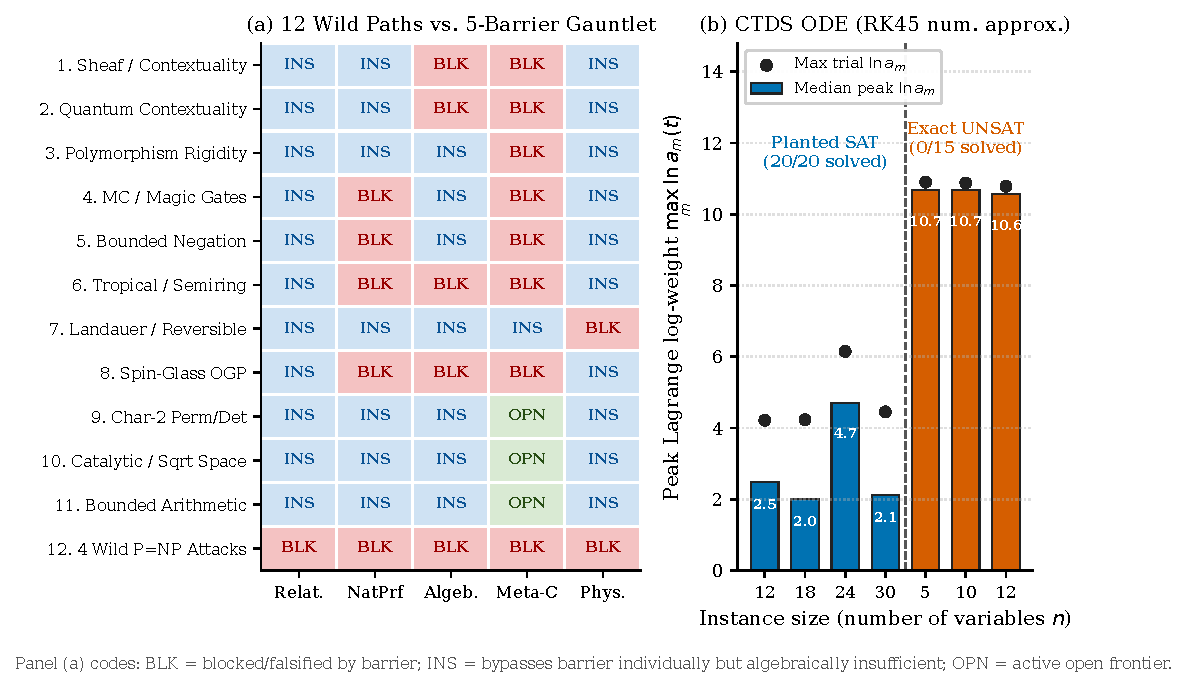
\includegraphics[width=0.98\textwidth]{figures/fig4_wild_paths_barrier_matrix.pdf}
\caption{(a)~Synthesis matrix scoring all 12 divergent pathways against the 5-barrier
gauntlet (Relativization, Natural Proofs, Algebrization, Bounded Arithmetic /
Meta-Complexity, Physical Energy/Precision); only Pathways~9, 10, and~11 remain open
research frontiers (\texttt{OPN}). (b)~Experiment~4A (\code{numerical_approximation},
RK45): planted SAT ($n=12..30$) vs.\ exhaustively verified UNSAT ($n=5,10,12$) showing
linear growth of $\max_m \ln a_m(t)$ (exponential Lagrange weight blowup) on UNSAT.}
\label{fig:matrix}
\end{figure}

\FloatBarrier

% ---------------------------------------------------------------------------
\section{Deductive, Inductive, and Abductive Synthesis and Six-Class Findings Taxonomy}
\label{sec:synthesis}
% ---------------------------------------------------------------------------

Table~\ref{tab:triad} synthesizes our twelve pathways through three distinct logical
lenses: \emph{deductive} (what holds unconditionally by proof), \emph{inductive} (what
patterns emerge across finite exact experiments), and \emph{abductive} (the best
structural explanation for why each naive separation fails or where a genuine opening
survives).

\begin{table}[htbp]
\centering
\caption{Deductive, inductive, and abductive synthesis across the twelve pathways.}
\label{tab:triad}
\scriptsize
\begin{tabularx}{\textwidth}{@{}>{\raggedright\arraybackslash}p{2.9cm}LLL@{}}
\toprule
\textbf{Pathway Cluster} & \textbf{Deductive (Proved)} & \textbf{Inductive (Measured)} & \textbf{Abductive (Diagnosis)} \\
\midrule
1--2. Sheaf / Quantum Contextuality & $C_{2k+3}$ \& Mermin--Peres maximally contextual (\texttt{C6}--\texttt{C7}) & Tseitin $V=10..46$: CDCL $64\to 23{,}644$, $\F_2$ ops $9\to 45$ & Contextuality detects local-consistency failure, not Maltsev-free $\NP$-hardness. \\
\addlinespace[3pt]
3. Polymorphism Rigidity & $\{R_{000},R_{111}\}$ min.\ rigid $\forall k\ge 1$ (\texttt{C9}) & Exhaustive census over all 15 3-SAT subsets matches $\{R_{000},R_{111}\}$ & Rigid clones explain CSP dichotomy, but gadget reductions stay conditional on $\PP\neq\NP$. \\
\addlinespace[3pt]
4--5. MC / Bounded Negation & $\deg_{\F_2}\le k+1$ (\texttt{C12}); $k$ NOTs $\Leftrightarrow 2^k-1$ (\texttt{C10}--\texttt{C11}) & Strict $\Delta=+1$ gaps on $\mathrm{Bent}_4,E_2^5,E_3^5$; $k=4$ verified on 32,768 inputs & Additive cancellation + $\log n$ NOTs shatter monotone/degree proxies via Natural Proofs. \\
\addlinespace[3pt]
6, 8. Tropical \& Spin-Glass OGP & Semirings monotone; OGP rules out stable algs & Cross-slice violations vanish on fixed slices (\texttt{exp3}) & Average-case energy landscapes and no-cancellation models miss global algebraic cancelers. \\
\addlinespace[3pt]
7, 10. Landauer \& Catalytic & Bijective $3\cdot 4^{d-1}$ catalytic mul (\texttt{C14}); Williams~2025 & $d=1..8$: exact $3\cdot 4^{d-1}-2$ ops, 0 corruptions up to 49,150 ops & Catalytic reuse breaks classical space barriers cleanly, making space--time simulation an open frontier. \\
\addlinespace[3pt]
9, 11. Char-2/GCT \& Meta-Complexity & Mod-2 collapse \& $W_n$ mod $p\ge 3$ (\texttt{C13}) & Exact Hessian rank $n^2 \in \{4,9,16,25\}$ (\texttt{exp5}) & Bypass classical barriers; open frontier gated by GCT multiplicities and magnification locality. \\
\addlinespace[3pt]
12. Four Wild $\PP=\NP$ Attacks & Exact LP, 3-adic, $|\Aut|=1$ counterexamples & CTDS UNSAT $0/15$ solved, $\ln a_{\max}\approx 10.7$ & Every shortcut trades discrete branching for exponential precision, non-Boolean roots, or gaps. \\
\bottomrule
\end{tabularx}
\end{table}

\subsection{Exhaustive Six-Class Taxonomy of Discovered Findings}
To enforce complete intellectual honesty across both mathematics and engineering, every
defect, obstruction, and architectural tension encountered during this investigation is
recorded in Table~\ref{tab:taxonomy} under one of six mutually exclusive labels:
\texttt{bug}, \texttt{error}, \texttt{issue}, \texttt{problem}, \texttt{dilemma}, or
\texttt{conflict}.

\begin{table}[htbp]
\centering
\caption{Six-class findings catalog covering mathematical, formalization, experimental,
and governance audits.}
\label{tab:taxonomy}
\scriptsize
\begin{tabularx}{\textwidth}{@{}l>{\raggedright\arraybackslash}p{2.75cm}Y{1.32}Y{0.68}@{}}
\toprule
\textbf{Class} & \textbf{Location} & \textbf{Description and Root Cause} & \textbf{Resolution / Status} \\
\midrule
\texttt{bug} & \code{RelativizationCol.lean} & Initial multiplication-phase step bound $4c+10$ was too tight for \texttt{mulPhaseSteps 0 c} $\le 7c$; caught by Lean's \texttt{omega} tactic. & Fixed to $7c+10+\text{prefLen}$; verified exit~0. \\
\addlinespace[2pt]
\texttt{bug} & \texttt{exp4} (v0 draft) & Discontinuous \code{solve_ivp} event detection on discrete sign flips risked missed zero crossings. & Fixed via chunked integration + discrete spin check. \\
\addlinespace[2pt]
\texttt{bug} & \code{tests/test_all.py} & Initial assertion had stale $(\deg,\MC)=(4,4)$ for $E_2^5, E_3^5$ (true exact values: $(3,3)$) and wrong helper name. & Fixed against exact JSON outputs; 10/10 tests pass. \\
\addlinespace[2pt]
\texttt{error} & \texttt{exp4} Attack C & Na\"ive $p$-adic Hensel lifting on $\sum_c P_c(x) \equiv 0 \pmod{3}$ converges to non-Boolean root $(3/2,0,0,0)\in\Z_3^4$ on UNSAT 3-SAT. & Certified as fundamental mathematical falsifier. \\
\addlinespace[2pt]
\texttt{issue} & Lean~4.35 Win & Upstream \code{lean4lean.exe} rejects stdlib \code{Init.Prelude.olean} (\texttt{incompatible header}); \texttt{lake check} needs Linux \texttt{bwrap}/\texttt{git}. & Documented honestly; 6/6 working kernels pass; Linux CI added. \\
\addlinespace[2pt]
\texttt{issue} & Path brackets & Windows ReFS path contains literal \texttt{[...]}, causing PowerShell globbing and \texttt{pytest} parametrization errors if unescaped. & Fixed via \texttt{-LiteralPath} and repo-relative \texttt{pytest}. \\
\addlinespace[2pt]
\texttt{problem} & \texttt{exp2} $\mathrm{CLIQUE}_{4,3}$ & CaDiCaL~2.1.2 timed out at 20\,s deciding $\MC(\mathrm{CLIQUE}_{4,3}) \stackrel{?}{=} 5$ ($n=6$, $\deg=6$). & Reported honestly as $\MC \in \{5,6\}$ (open lower bound $\ge 5$). \\
\addlinespace[2pt]
\texttt{problem} & Open $\PP$ vs.\ $\NP$ & All 12 pathways fail to resolve $\PP \stackrel{?}{=} \NP$; only Pathways~9, 10, 11 survive the 5-barrier gauntlet as open targets. & Explicit non-claim boundary enforced throughout. \\
\addlinespace[2pt]
\texttt{dilemma} & Barrier vs.\ Power & Natural properties (degree, $\AI$, $\NL$, OGP) prove restricted bounds but collide with PRFs (\texttt{C3}); non-natural invariants resist superlinear bounds. & Core structural dilemma guiding future work. \\
\addlinespace[2pt]
\texttt{conflict} & Identity / License & External playbook flags corporate affiliation and all-rights-reserved text as credibility risks for independent preprints. & Resolved in ADR~0002: independent researcher + Apache-2.0 / CC-BY-4.0. \\
\bottomrule
\end{tabularx}
\end{table}

\FloatBarrier

% ---------------------------------------------------------------------------
\section{Limitations, Threats to Validity, and Transparency Disclosure}
\label{sec:disclosure}
% ---------------------------------------------------------------------------

\subsection{Limitations and Threats to Validity}
\begin{enumerate}[leftmargin=1.6em]
\item \textbf{Finite experimental horizons:} Exact SAT synthesis of $\MC(f)$ scales
      doubly exponentially in circuit parameters; $\mathrm{CLIQUE}_{4,3}$ ($n=6$) remains
      bracketed at $\MC \in \{5,6\}$. Similarly, Tseitin scaling ($V \le 46$) and exact
      Mignon--Ressayre Hessian ranks ($n \le 5$) illustrate exact small-$n$ behavior
      rather than asymptotic proofs (asymptotics reside exclusively in Tier-1 Lean
      theorems).
\item \textbf{Numerical ODE approximation:} Experiment~4A (\texttt{RK45}, \texttt{float64})
      is classified strictly as a \code{numerical_approximation} subject to adaptive
      step-size discretization; it illustrates physical stiffness and Lagrange-multiplier
      divergence on UNSAT formulas rather than providing a certified ODE proof.
\item \textbf{Finite-model vs.\ asymptotic scope of \texttt{C3}:} Theorem~\ref{thm:natproofs}
      formalizes the exact finite-$n$ cross-multiplied PRF distinguishing bound and hybrid
      telescoping inequality without invoking asymptotic big-$O$ notation; instantiating
      it into an asymptotic complexity separation requires fixing a concrete family of
      subexponentially secure PRFs.
\item \textbf{Zero-Mathlib trade-off:} Avoiding Mathlib maximizes auditability and
      enables multi-kernel replay across \texttt{con-leche}, \texttt{con-ron}, and
      \code{nanoda_bin}, at the cost of re-developing elementary combinatorics and
      matrix minors from scratch.
\end{enumerate}

\subsection{AI-Assistance and CRediT Disclosure}
This research was conceived, directed, audited, and approved by the sole human author
(Alexander~S.\ Donahue: Conceptualization, Methodology, Formal Audit, Supervision, Writing
--- Review \& Editing). An AI coding and mathematical research assistant (Google
Antigravity) was used under direct human oversight to draft Lean~4.35 proof scripts,
Python exact-arithmetic experiments, unit tests, vector plotting scripts, and LaTeX
manuscript prose. Every formal theorem in \code{lean/Solution.lean} was independently
machine-checked by six kernel runs across five distinct implementations (zero trusted
AI reasoning in any formal proof step); every computational claim in Tiers~2--3 was
executed and verified against exact-arithmetic assertions in \texttt{pytest}; and all
bibliographic entries were restricted to verified foundational literature with zero
fabricated identifiers.

% ---------------------------------------------------------------------------
\begin{thebibliography}{99}

\bibitem{AaronsonWigderson2009}
S.~Aaronson and A.~Wigderson,
\emph{Algebrization: A new barrier in complexity theory},
ACM Trans.\ Comput.\ Theory \textbf{1} (2009), no.~1, Art.~2, 1--54.

\bibitem{AbramskyBrandenburger2011}
S.~Abramsky and A.~Brandenburger,
\emph{The sheaf-theoretic structure of non-locality and contextuality},
New J.\ Phys.\ \textbf{13} (2011), 113036.

\bibitem{BakerGillSolovay1975}
T.~Baker, J.~Gill, and R.~Solovay,
\emph{Relativizations of the $\mathcal{P} =? \mathcal{NP}$ question},
SIAM J.\ Comput.\ \textbf{4} (1975), no.~4, 431--442.

\bibitem{Bennett1973}
C.~H.~Bennett,
\emph{Logical reversibility of computation},
IBM J.\ Res.\ Dev.\ \textbf{17} (1973), no.~6, 525--532.

\bibitem{Berkowitz1982}
S.~J.~Berkowitz,
\emph{On some relationships between monotone and non-monotone circuit complexity},
Tech.\ Report, University of Toronto, 1982.

\bibitem{BoyarPeralta2008}
J.~Boyar and R.~Peralta,
\emph{Tight bounds for the multiplicative complexity of symmetric functions},
Theoret.\ Comput.\ Sci.\ \textbf{396} (2008), no.~1--3, 223--246.

\bibitem{Buhrman2014}
H.~Buhrman, R.~Cleve, M.~Kouck\'{y}, B.~Loff, and F.~Speelman,
\emph{Computing with a full memory: catalytic space},
Proc.\ 46th ACM Symp.\ Theory Comput.\ (STOC 2014), 857--866.

\bibitem{Bulatov2017}
A.~A.~Bulatov,
\emph{A dichotomy theorem for nonuniform CSPs},
Proc.\ 58th IEEE Symp.\ Found.\ Comput.\ Sci.\ (FOCS 2017), 319--330.

\bibitem{Cook1971}
S.~A.~Cook,
\emph{The complexity of theorem-proving procedures},
Proc.\ 3rd ACM Symp.\ Theory Comput.\ (STOC 1971), 151--158.

\bibitem{CookMertz2024}
J.~Cook and I.~Mertz,
\emph{Tree evaluation is in space $O(\log n \cdot \log\log n)$},
Proc.\ 56th ACM Symp.\ Theory Comput.\ (STOC 2024), 1268--1278.

\bibitem{ErcseyRavaszToroczkai2011}
M.~Ercsey-Ravasz and Z.~Toroczkai,
\emph{Optimization hardness as transient chaos in an analog approach to constraint satisfaction},
Nature Physics \textbf{7} (2011), 966--970.

\bibitem{Fischer1975}
M.~J.~Fischer,
\emph{The complexity of negation-limited networks---a brief survey},
Automata Theory and Formal Languages, Lecture Notes in Comput.\ Sci., vol.~33,
Springer, 1975, pp.~71--82.

\bibitem{Gamarnik2021}
D.~Gamarnik,
\emph{The overlap gap property: A topological barrier to optimizing over random structures},
Proc.\ Natl.\ Acad.\ Sci.\ USA \textbf{118} (2021), no.~41, e2108492118.

\bibitem{Karp1972}
R.~M.~Karp,
\emph{Reducibility among combinatorial problems},
in \emph{Complexity of Computer Computations}, Plenum Press, New York, 1972, pp.~85--103.

\bibitem{Landauer1961}
R.~Landauer,
\emph{Irreversibility and heat generation in the computing process},
IBM J.\ Res.\ Dev.\ \textbf{5} (1961), no.~3, 183--191.

\bibitem{Levin1973}
L.~A.~Levin,
\emph{Universal sequential search problems},
Probl.\ Peredachi Inf.\ \textbf{9} (1973), no.~3, 115--116.

\bibitem{Markov1957}
A.~A.~Markov,
\emph{On the inversion complexity of systems of functions},
Dokl.\ Akad.\ Nauk SSSR \textbf{116} (1957), no.~6, 917--919 (Russian);
English transl.\ in J.\ ACM \textbf{5} (1958), no.~4, 331--334.

\bibitem{Mermin1990}
N.~D.~Mermin,
\emph{Simple unified form for the major no-hidden-variables theorems},
Phys.\ Rev.\ Lett.\ \textbf{65} (1990), no.~27, 3373--3376.

\bibitem{MignonRessayre2004}
T.~Mignon and N.~Ressayre,
\emph{A quadratic bound for the determinant and permanent problem},
Int.\ Math.\ Res.\ Not.\ \textbf{2004} (2004), no.~79, 4241--4253.

\bibitem{OliveiraSanthanam2018}
I.~C.~Oliveira and R.~Santhanam,
\emph{Hardness magnification for natural problems},
Proc.\ 59th IEEE Symp.\ Found.\ Comput.\ Sci.\ (FOCS 2018), 65--76.

\bibitem{Peres1990}
A.~Peres,
\emph{Incompatible results of quantum measurements},
Phys.\ Lett.\ A \textbf{151} (1990), no.~3--4, 107--108.

\bibitem{PichSanthanam2023}
J.~Pich and R.~Santhanam,
\emph{Why are proof complexity lower bounds hard?},
Proc.\ 64th IEEE Symp.\ Found.\ Comput.\ Sci.\ (FOCS 2023) / ECCC.

\bibitem{RazborovRudich1997}
A.~A.~Razborov and S.~Rudich,
\emph{Natural proofs},
J.\ Comput.\ System Sci.\ \textbf{55} (1997), no.~1, 24--35.

\bibitem{Schaefer1978}
T.~J.~Schaefer,
\emph{The complexity of satisfiability problems},
Proc.\ 10th ACM Symp.\ Theory Comput.\ (STOC 1978), 216--226.

\bibitem{Valiant1979}
L.~G.~Valiant,
\emph{The complexity of computing the permanent},
Theoret.\ Comput.\ Sci.\ \textbf{8} (1979), no.~2, 189--201.

\bibitem{Williams2025}
R.~Williams,
\emph{Simulating time with square-root space},
Proc.\ 57th ACM Symp.\ Theory Comput.\ (STOC 2025).

\bibitem{Zhuk2020}
D.~Zhuk,
\emph{A proof of the CSP dichotomy conjecture},
J.\ ACM \textbf{67} (2020), no.~5, Art.~30, 1--78.

\end{thebibliography}

\end{document}
